\documentclass{unicam_thesis}
\usepackage[utf8]{inputenc}
\usepackage{listings}
\usepackage{braket}
\usepackage[backend=bibtex]{biblatex}
\usepackage[automake,toc,acronyms,nonumberlist, nopostdot]{glossaries}
\usepackage{mathabx}
\usepackage{amsthm}
\usepackage{graphicx} 
\usepackage{tikz}  
\usetikzlibrary{angles, quotes, quantikz, positioning, arrows.meta, calc, automata, positioning, backgrounds, fit, shapes.geometric}
\usepackage{booktabs}     
\usepackage{amsthm}
\usepackage{adjustbox}
\usepackage{amssymb}
\usepackage[utf8]{inputenc}
\usepackage[T1]{fontenc}
\usepackage{lmodern}
\usepackage[nottoc]{tocbibind}
\usepackage{hyperref}
\usepackage{braket}
\usepackage{wasysym}
\usepackage[english]{babel}
\usepackage{csquotes}
\usepackage{tabularx}
\usepackage{array}
\usepackage{algorithm}
\usepackage{algpseudocode}
\usepackage{enumitem}
\usepackage{subcaption}
\captionsetup{compatibility=false}

\theoremstyle{plain}
\newtheorem{theorem}{Theorem}[section]
\newtheorem{lemma}{Lemma}[section]
\newtheorem{corollary}{Corollary}[section]
\newtheorem{proposition}{Proposition}[section]
\newtheorem{conjecture}{Conjecture}[section]
\newtheorem{assumption}{Assumption}[section]

\theoremstyle{definition}
\newtheorem{definition}{Definition}[section]
\newtheorem{example}{Example}[section]
\newtheorem{exercise}{Exercise}[section]
\newtheorem{concept}{Concept}[section]

\theoremstyle{remark}
\newtheorem*{remark}{Remark}
\newtheorem{observation}{Observation}[section]
\newtheorem{notation}{Notation}[section] 

\tikzset{rejecting/.style={circle, draw, red, dashed}}

\makeglossaries
\loadglsentries[acronym]{myglossaries}

\title{Towards a Unified Taxonomy and Architecture-Independent Quantum Circuit Compilation for Quantum Finite Automata}

\university{Universit\`a degli Studi di Camerino}
\school{Scienze e Tecnologie}
\course{Laurea in Informatica (Classe L-31)}


\author{Marta Musso}
\advisor{Prof.\ Dr.\ Michele Loreti\\Prof.\ Dr.\ Marcello Bonsangue}
%\coadvisor2{}
\academicyear{2024/2025}
\matricola{122360}

\graphicspath{{Screenshot/},{Pictures/},{API/},{Source/}}
\addbibresource{biblio.bib}
\begin{document}

\maketitle
\begin{abstract} {
    As quantum computing matures, concise models are needed to connect its theoretical foundations with practical implementations.  
    Quantum finite automata fulfil this role by extending the well-known framework of classical finite automata into the quantum domain, offering a compact setting in which to study finite-memory quantum behaviour.  
    
    This thesis first revisits the essential background on both quantum information and classical automata, establishing a common language for readers from either field.  
    It then delivers a comprehensive literature review that consolidates the many quantum finite automata variants introduced over the last three decades and arranges them in a unified, consistently named taxonomy.  
    Building on that organisation, the work presents a compilation algorithm that translates the widely studied measure-once and measure-many quantum finite automata models into architecture-independent quantum-circuit templates, thereby bridging abstract automaton descriptions with executable gate-level designs.
    
    Viewed more broadly, this study contributes a computer-science perspective on the quantum landscape and offers an accessible entry point for further research in quantum software by promoting circuit-level abstraction and enabling systematic comparison of different designs.
}

\noindent\textbf{Keywords: Quantum finite automata, automata theory, quantum information, quantum computing, quantum circuits, quantum compilation.}
\end{abstract}
\newpage


\tableofcontents

%\lstlistoflistings
%\listoffigures
%\listoftables

\chapter{Introduction}
\label{chap:introduction}

The accelerating development of quantum computing has sparked a parallel evolution in theoretical models that aim to describe and harness quantum behaviour within computational frameworks. As researchers strive to reconcile physical limitations with algorithmic expressiveness, the study of \glspl{qfa} has emerged as a promising direction. These automata extend the well-established framework of classical finite automata into the quantum domain, yielding models that are minimalistic in structure yet rich in quantum phenomena.

\Glspl{qfa} are particularly attractive due to their finite memory constraints, making them ideal for investigating foundational questions in quantum computational theory and exploring efficient recognisers for regular and near-regular languages. Moreover, their simplicity renders them amenable to physical implementation on \gls{nisq} devices, where full-scale quantum algorithms remain impractical. Despite this promise, the diversity of \gls{qfa} models has led to a fragmented landscape. Disparate notations, inconsistent terminologies, and varied acceptance criteria have made it difficult to compare models, reason about their capabilities, or implement them in a unified framework.

This thesis addresses these challenges through two major contributions. First, it provides a coherent and systematic taxonomy of \glspl{qfa}. Drawing on over three decades of research, the thesis consolidates the principal families of \gls{qfa} into a unified nomenclature and identifies key relationships between models. This classification is not merely pedagogical—it lays the foundation for rigorous analysis and comparison of expressive power, closure properties, and language recognition capabilities.

Second, the thesis introduces a compilation framework that transforms high-level descriptions of \glspl{mo-1qfa} and \glspl{mm-1qfa}, into executable quantum circuits. These circuits are constructed to preserve the semantics of the original automaton, enabling formal verification and direct deployment on quantum hardware. The compilation process is structured into two phases: symbolic template generation, which defines the automaton’s logical structure for inputs of fixed length, and operator instantiation, which assigns concrete unitary transformations to each input-driven transition.

The remainder of the thesis is organised as follows. Chapter~\ref{chap:background} reviews the necessary background in classical automata theory and quantum information science. Chapter~\ref{chap:quantum-finite-automata} delves into the taxonomy of \glspl{qfa}, presenting detailed definitions and formal properties of each model. Chapter~\ref{chap:automata-to-circuits} details the circuit compilation framework, with examples illustrating how abstract automata are translated into gate-level designs. The thesis concludes in Chapter~\ref{chap:conclusion} by summarising the contributions and findings, along with a discussion of potential extensions to more powerful models and reflections on the role of \glspl{qfa} in the broader context of quantum software engineering.



\chapter{Background}  
\label{chap:background}
This chapter provides the theoretical and mathematical foundations that connect classical models of computation with quantum information theory, structured around three central domains: classical automata theory, finite-dimensional quantum mechanics, and the gate-based framework of quantum circuits.

We begin by reviewing the algebra of formal languages and the computational limitations and expressiveness of \glspl{cfa}. The section formalises \glspl{dfa}, \glspl{nfa}, \glspl{pfa}, and \glspl{2fa}, examining their closure properties, characterisation of \glspl{reg}, and algebraic structure, which together form a foundational framework for the study of automaton-based computation \cite{hopcroft2001introduction}.

Next, we present the finite-dimensional postulates of non-relativistic quantum mechanics. This section covers the fundamental ideas of superposition, entanglement, the probabilistic nature of quantum measurement, and the encoding of information in qubits and quantum states in the context of quantum dynamics, which includes unitary evolution governed by the Schrödinger equation and the handling of decoherence and open systems via density matrices.
The exposition follows the axiomatic approach developed by Dirac and von Neumann \cite{dirac1981principles,von2018mathematical}, with particular emphasis on features pertinent to quantum automata, including projective measurements, the no-cloning theorem, and the compositional structure of subsystems \cite{wootters1982single}.

The gate-based circuit model of quantum computation is covered in the last section. It reviews common quantum gates, families of circuits (including parameterised and measurement-based circuits), the implementation of quantum algorithms, and the decomposition of arbitrary unitary operations into standard gate sets \cite{weinberg1995quantum,fedoriaka2025decomposition}. The circuit-level realisation of \glspl{qfa} covered in later chapters is based on these ideas.

Together, these three pillars form the theoretical foundation upon which the thesis develops its unified treatment of \glspl{qfa}, their taxonomy, and their compilation into executable circuits.

\section{\glsentrylongpl{cfa} and Formal Languages}\label{sec:cfa-languages}

Finite automata occupy the lowest computational tier: machines whose
memory is bounded by a constant independent of the input length.  They
nevertheless underpin lexical analysis, model checking and the design
of communication protocols
\cite{AhoHopcroftUllman1974,Sipser2012}.  This section moves from
general language–grammar notions to four concrete automaton models,
highlighting their historical development, formal properties and
representative examples.

\subsection{Languages, Grammars and Regularity}\label{subsec:foundations}

Finite automata study begins with the algebra of words.  The discussion
below moves from the atomic notion of an alphabet to the structural
power of regular grammars, concluding with Kleene’s correspondence
between grammars, expressions and machines.

\begin{definition}[Alphabet]\label{def:alphabet}
A non-empty finite set $\Sigma$ of symbols is called an alphabet
\cite{HopcroftUllman1979}.
\end{definition}

\begin{definition}[String and Concatenation]\label{def:string}
A string, or word, over $\Sigma$ is a finite sequence
$w=a_{1}a_{2}\dots a_{n}$ with $a_{i}\in\Sigma$.  
The empty word is denoted $\varepsilon$.  
Concatenation $u\cdot v$ appends the sequence of $v$ to $u$
\cite{HopcroftUllman1979}.
\end{definition}

\begin{notation}
The set of all words over $\Sigma$ forms the free monoid
$\Sigma^{\ast}$ under concatenation with identity $\varepsilon$
\cite{HopcroftUllman1979}.
\end{notation}

\begin{definition}[Formal Language]\label{def:language}
Any subset $L\subseteq\Sigma^{\ast}$ is a language
\cite{HopcroftUllman1979}.
\end{definition}

\begin{concept}[Regular Grammar]\label{concept:regular-grammar}
A type-3 grammar in Chomsky’s hierarchy generates the regular languages
\cite{Chomsky1959}.
\end{concept}

\begin{theorem}[Kleene Correspondence]\label{thm:kleene}
The following families coincide:
\begin{enumerate}
  \item languages generated by type-3 grammars,
  \item languages denoted by regular expressions,
  \item languages recognised by \glspl{cfa}.
\end{enumerate}
\cite{Kleene1956}
\end{theorem}

\begin{proposition}[Closure of Regular Languages]\label{prop:closure}
Let ${\cal R}$ denote the class of regular languages.  
If $L_{1},L_{2}\in{\cal R}$ then so are
$L_{1}\cup L_{2}$, $L_{1}\cap L_{2}$, $\overline{L_{1}}$,
$L_{1}\,L_{2}$ and $L_{1}^{\ast}$  
\cite{HopcroftUllman1979}.
\end{proposition}

\begin{example}[Simple Regular Language]\label{ex:reg-lang}
For $\Sigma=\{0,1\}$ the set
$L=\{w\in\Sigma^{\ast}\mid w\text{ ends in }1\}$ is regular because it
is described by the regular expression $\Sigma^{\ast}1$
\cite{HopcroftUllman1979}.
\end{example}

\begin{observation}\label{obs:why-regular-matters}
Regular languages admit linear-time membership tests and deterministic
finite-state representations; hence they are widely used in lexical
tokenisers and hardware controllers \cite{AhoHopcroftUllman1974}.
\end{observation}

\subsection{Deterministic Finite Automata}\label{subsec:dfa}

Deterministic machines give the clearest computational intuition: at
every step the next state is uniquely determined by the current state
and the scanned symbol \cite{HopcroftUllman1979}.

\begin{definition}[Deterministic Finite Automaton]\label{def:dfa}
A \gls{dfa} is the quintuple
$M=(Q,\Sigma,\delta,q_{0},F)$ with
$\delta\colon Q{\times}\Sigma\to Q$,
$q_{0}\in Q$ and $F\subseteq Q$
\cite{HopcroftUllman1979}.
\end{definition}

\begin{proposition}[Unique Computation Path]\label{prop:dfa-path}
For every $w\in\Sigma^{\ast}$ the extended map
$\hat{\delta}(q,\varepsilon)=q$ and
$\hat{\delta}(q,aw)=\hat{\delta}(\delta(q,a),w)$
produces exactly one path in $M$
\cite{HopcroftUllman1979}.
\end{proposition}

\begin{theorem}[Myhill–Nerode]\label{thm:mn-dfa}
A language is regular if and only if the right-invariant relation
$x\sim_{L}y\Longleftrightarrow
\forall z\in\Sigma^{\ast}\colon xz\in L\Leftrightarrow yz\in L$
has finitely many equivalence classes
\cite{Nerode1958}.
\end{theorem}

\begin{example}[Even $a$’s]\label{ex:dfa-even}
Figure~\ref{fig:dfa-even-a} shows the \gls{dfa} recognising
$L=\{w\mid \text{the number of }a\text{ is even}\}$
\cite{HopcroftUllman1979}.
\end{example}

\begin{observation}[Practical role]\label{obs:dfa-app}
\glspl{dfa} underlie lexical tokenisers, hardware controllers and regex
engines that insist on linear-time, deterministic matching
\cite{AhoHopcroftUllman1974}.
\end{observation}

\begin{figure}[H]
    \centering
    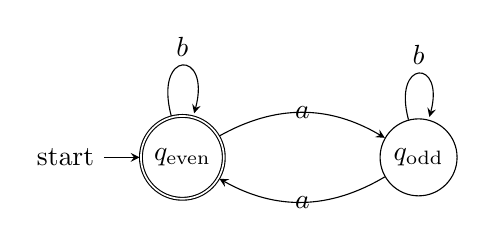
\begin{tikzpicture}[->,>=stealth,node distance=30mm]
      \node[state,initial,accepting] (qe) {$q_{\mathrm{even}}$};
      \node[state]                   (qo) [right of=qe] {$q_{\mathrm{odd}}$};
      \path (qe) edge[loop above] node {$b$} (qe)
            (qo) edge[loop above] node {$b$} (qo)
            (qe) edge[bend left]  node {$a$} (qo)
            (qo) edge[bend left]  node {$a$} (qe);
    \end{tikzpicture}
    \caption{\gls{dfa} recognising words with an even number of $a$’s
    \cite{HopcroftUllman1979}.}
    \label{fig:dfa-even-a}
\end{figure}

\subsection{Nondeterministic Finite Automata}\label{subsec:nfa}

Nondeterminism lets an automaton explore many futures simultaneously,
shrinking state space at the cost of branching semantics
\cite{RabinScott1959}.

\begin{definition}[Nondeterministic Finite Automaton]\label{def:nfa}
A \gls{nfa} is $M=(Q,\Sigma,\delta,q_{0},F)$ with
$\delta\colon Q{\times}\Sigma\to\mathcal{P}(Q)$
\cite{RabinScott1959}.
\end{definition}

\begin{lemma}[Acceptance Criterion]\label{lem:nfa-accept}
$M$ accepts $w$ iff there exists a sequence
$q_{0}\to q_{1}\to\dots\to q_{|w|}\in F$ such that
$q_{i+1}\in\delta(q_{i},w_{i+1})$
\cite{HopcroftUllman1979}.
\end{lemma}

\begin{theorem}[Subset Construction]\label{thm:subset}
Every \(n\)-state \gls{nfa} has an equivalent \gls{dfa}
with at most \(2^{n}\) states
\cite{RabinScott1959}.
\end{theorem}

\begin{example}[Length-one words]\label{ex:nfa-length1}
The \gls{nfa} in Figure~\ref{fig:nfa-figure} accepts
$\Sigma^{1}$ using $\epsilon$-transitions
\cite{RabinScott1959}.
\end{example}

\begin{observation}[Succinctness]\label{obs:nfa-size}
There exist languages whose minimal \gls{nfa} is linear in $n$ while
every equivalent \gls{dfa} requires $2^{n}$ states
\cite{AhoHopcroftUllman1974}.
\end{observation}

\begin{figure}[H]
    \centering
    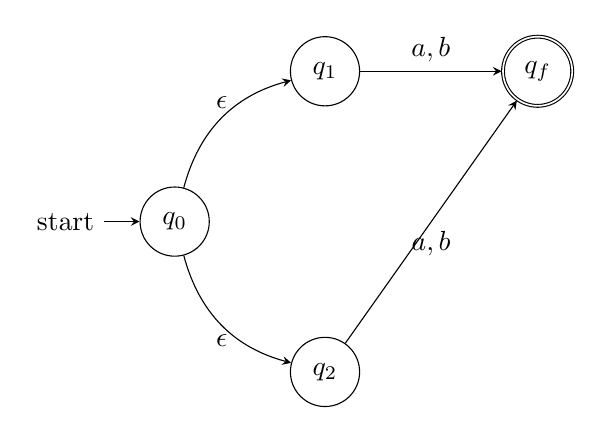
\begin{tikzpicture}[->,>=stealth,node distance=27mm]
      \node[state,initial] (q0) {$q_{0}$};
      \node[state]         (q1) [above right of=q0] {$q_{1}$};
      \node[state]         (q2) [below right of=q0] {$q_{2}$};
      \node[state,accepting] (qf) [right of=q1] {$q_{f}$};
      \path (q0) edge[bend left]  node[above] {$\epsilon$} (q1)
            (q0) edge[bend right] node[below] {$\epsilon$} (q2)
            (q1) edge node[above] {$a,b$} (qf)
            (q2) edge node[below] {$a,b$} (qf);
    \end{tikzpicture}
    \caption{\gls{nfa} accepting all words of length one
    \cite{RabinScott1959}.}
    \label{fig:nfa-figure}
\end{figure}

\subsection{Probabilistic Finite Automata}\label{subsec:pfa}

By weighting transitions with probabilities, \glspl{pfa} capture
one-way finite-state stochastic processes
\cite{Rabin1963}.

\begin{definition}[Probabilistic Finite Automaton]\label{def:pfa}
A \gls{pfa} is
$M=(Q,\Sigma,\{\delta(a)\}_{a\in\Sigma},\mathbf{i},F)$
where each
$\delta(a)\in[0,1]^{Q\times Q}$ is row-stochastic and
$\mathbf{i}\in[0,1]^{Q}$ is an initial distribution
\cite{Rabin1963}.
\end{definition}

\begin{concept}[Cut-point Language]\label{concept:cutpoint}
Given $\lambda\in[0,1]$,
$L(M,\lambda)=\{w\mid \Pr_{M}(w)>\lambda\}$ is the cut-point language
of $M$ \cite{Rabin1963}.
\end{concept}

\begin{theorem}[Bounded-error Regularity]\label{thm:pfa-bounded}
If \(\lambda\) is isolated (bounded error) then
\(L(M,\lambda)\) is regular \cite{Paz1971}.
\end{theorem}

\begin{proposition}[Undecidability]\label{prop:pfa-undec}
Equivalence and emptiness are undecidable for unbounded-error
\glspl{pfa} \cite{Paz1971}.
\end{proposition}

\begin{example}[Unary PFA]\label{ex:pfa-unary}
Figure~\ref{fig:pfa-figure} shows a \gls{pfa} over $\{a\}$ accepting
$a^{k}$ for $k\ge2$ with cut-point $\lambda=0.5$
\cite{Rabin1963}.
\end{example}

\begin{observation}[Historical note]\label{obs:pfa-history}
\glspl{pfa} foreshadow probabilistic Turing machines and
finite-memory Markov models used in speech recognition
\cite{Rabin1963,Paz1971}.
\end{observation}

\begin{figure}[H]
    \centering
    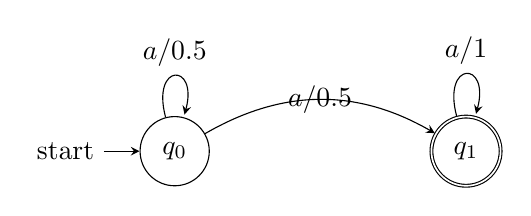
\begin{tikzpicture}[->,>=stealth,node distance=37mm]
      \node[state,initial] (q0) {$q_{0}$};
      \node[state,accepting] (q1) [right of=q0] {$q_{1}$};
      \path (q0) edge[loop above] node {$a/0.5$} (q0)
            (q0) edge[bend left]  node {$a/0.5$} (q1)
            (q1) edge[loop above] node {$a/1$} (q1);
    \end{tikzpicture}
    \caption{\gls{pfa} that, with cut-point $\lambda=0.5$, recognises
    $\{a^{k}\mid k\ge 2\}$ \cite{Rabin1963}.}
    \label{fig:pfa-figure}
\end{figure}

%-----------------------------------------------------------------------
% 4 Two-way finite-automata variants
%-----------------------------------------------------------------------
\subsection{Two-way variants}\label{subsec:two-way}

Allowing the tape head to reverse direction enriches operational
behaviour without extending expressive power beyond regular languages
\cite{Shepherdson1959}.

\begin{definition}[Two-way Head]\label{def:two-way-head}
On alphabet $\Sigma_{\Box}=\Sigma\cup\{\Box\}$ a head movement is
$d\in\{-1,0,1\}$, signifying left, stay, right
\cite{Shepherdson1959}.
\end{definition}

\begin{definition}[2DFA, 2NFA, 2PFA]\label{def:2dfa2nfa2pfa}
\begin{enumerate}
\item \gls{2dfa}: deterministic
$\delta\colon Q{\times}\Sigma_{\Box}\to Q{\times}\{-1,0,1\}$.
\item \gls{2nfa}: the same domain but $\delta$ returns a set of
state–move pairs \cite{RabinScott1959}.
\item \gls{2pfa}: for each input symbol a row-stochastic distribution
over state–move pairs \cite{Freivalds1982}.
\end{enumerate}
\end{definition}

\begin{theorem}[Expressive Power]\label{thm:two-way-reg}
Bounded-error \glspl{2pfa}, as well as \glspl{2dfa} and \glspl{2nfa},
recognise exactly the regular languages
\cite{Freivalds1982,Shepherdson1959}.
\end{theorem}

\begin{proposition}[Simulation Costs]\label{prop:two-way-cost}
Simulating an \(n\)-state \gls{2dfa} or \gls{2nfa} by a one-way
\gls{dfa} may incur \(2^{\mathcal{O}(n\log n)}\) states
\cite{Shepherdson1959,RabinScott1959}.  
A bounded-error \gls{2pfa} needs $\mathcal{O}(n^{2})$ states when
converted to a one-way \gls{pfa} \cite{DworkStockmeyer1992}.
\end{proposition}

\begin{example}[Sketch 2PFA]\label{ex:2pfa-sketch}
Figure~\ref{fig:2pfa-figure} illustrates a bounded-error
\gls{2pfa} \cite{Freivalds1982}.
\end{example}

\begin{observation}[Bidirectional processing]\label{obs:two-way-app}
Two-way automata model stream processors that reread data, a capability
used in text editors and network-protocol verification
\cite{Shepherdson1959}.
\end{observation}

\begin{figure}[H]
    \centering
    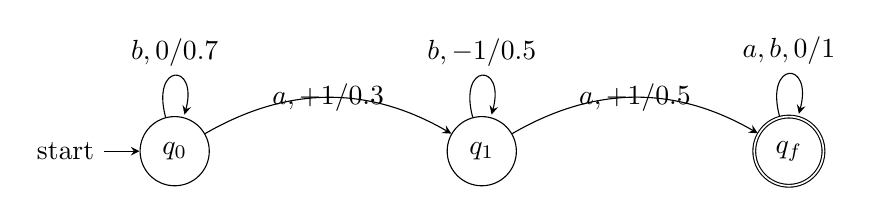
\begin{tikzpicture}[->,>=stealth,node distance=39mm]
      \node[state,initial] (q0) {$q_{0}$};
      \node[state]         (q1) [right of=q0] {$q_{1}$};
      \node[state,accepting] (qf) [right of=q1] {$q_{f}$};
      \path (q0) edge[loop above] node {$b,0/0.7$} (q0)
            (q0) edge[bend left] node {$a,+1/0.3$} (q1)
            (q1) edge[loop above] node {$b,-1/0.5$} (q1)
            (q1) edge[bend left] node {$a,+1/0.5$} (qf)
            (qf) edge[loop above] node {$a,b,0/1$} (qf);
    \end{tikzpicture}
    \caption{Sketch of a bounded-error \gls{2pfa}
    \cite{Freivalds1982}.}
    \label{fig:2pfa-figure}
\end{figure}

\section{Quantum Mechanics Foundations}
\label{sec:quantum-foundations}

\subsection{Qubits and Quantum States}
\label{subsec:qubits-and-quantum-states}


\subsection{Superposition and Entanglement}
\label{subsec:superposition-and-entanglement}

\subsection{Measurement and Probabilistic Outcomes}
\label{subsec:measurement-and-probabilistic-outcomes}
\subsection{Decoherence and Open Systems}
\label{subsec:decoherence-and-open-systems}

 
\subsection{Unitary Evolution and Quantum Dynamics}
\label{subsec:unitary-evolution-and-quantum-dynamics}
    
\section{Quantum Gates and Circuits}
\label{sec:quantum-gates-and-circuits}


\chapter{Quantum Finite Automata}
\label{chap:quantum-finite-automata}
%TODO: rewrite
\section{Basic Models of Quantum Finite Automata}
\label{sec:basic-models}
\subsection{\glsentrylong{moqfa}}
\label{sec:moqfa}
This section introduces the \glsentryfull{moqfa}, a quantum model in which the system evolves through unitary operations over the entire input and a single measurement is performed at the end. In the bounded error setting, the class of languages accepted by MO-QFAs coincides with the group languages (those accepted by group finite automata).

\subsubsection{Definition}
An MO-QFA is defined as a 5-tuple 
\[
M = (Q, \Sigma, \delta, q_0, F),
\]
where:
\begin{itemize}
  \item $Q$ is a finite set of states.
  \item $\Sigma$ is a finite input alphabet; an end-marker (e.g., $\$$) is appended to indicate the end of the input.
  \item $\delta: Q \times \Sigma \times Q \to \mathbb{C}$ is a transition function such that for all $q_1,q_2 \in Q$ and for every $\sigma \in \Sigma$, the unitary condition
  \[
  \sum_{q' \in Q} \delta(q_1, \sigma, q')\,\delta(q_2, \sigma, q')^* =
  \begin{cases}
    1, & \text{if } q_1 = q_2,\\[1mm]
    0, & \text{if } q_1 \neq q_2,
  \end{cases}
  \]
  holds.
  \item $q_0\in Q$ is the initial state.
  \item $F\subseteq Q$ is the set of accepting states.
\end{itemize}
The computation proceeds by applying the unitary transformations associated with the symbols of the input string, and only after reading the entire input is a projective measurement performed to decide acceptance.

\subsubsection{Accepted Strings}
For an input string $x\in\Sigma^*$, let
\[
|\Psi_x\rangle = U(x)|q_0\rangle,
\]
where $U(x)$ is the product of unitary matrices corresponding to the symbols of $x$. Denote by $P$ the projection onto the subspace spanned by the accepting states $F$. Then the acceptance probability is given by
\[
p_M(x) = \|P\,|\Psi_x\rangle\|^2.
\]
A string is accepted if $p_M(x)$ exceeds a designated cut-point (or, in the bounded error model, is separated from the cut-point by some margin $\epsilon>0$).

\subsubsection{Language Acceptance}
An MO-QFA is said to accept a language $L\subseteq\Sigma^*$ with cut-point $\lambda$ if
\[
x\in L \Longrightarrow p_M(x) > \lambda \quad \text{and} \quad x\notin L \Longrightarrow p_M(x) \le \lambda.
\]
In the bounded error scenario, there exists an $\epsilon>0$ such that for all $x\in L$, 
\[
p_M(x) \ge \lambda + \epsilon,
\]
and for all $x\notin L$,
\[
p_M(x) \le \lambda - \epsilon.
\]
It has been shown that, with bounded error, the languages recognized by MO-QFAs (often denoted by the class RMO) are exactly the group languages.

\subsubsection{Properties}
MO-QFAs exhibit several interesting properties:
\begin{itemize}
  \item \textbf{Closure Properties:} The class of languages accepted by MO-QFAs with bounded error is closed under inverse homomorphisms, word quotients, and Boolean operations (such as union and intersection), although it is not closed under arbitrary homomorphisms.
  \item \textbf{Decidability:} Equivalence of two MO-QFAs (i.e., whether they yield the same acceptance probabilities on all inputs) can be decided by transforming them into bilinear representations and applying known algorithms.
  \item \textbf{Simulation by Classical Models:} Every MO-QFA that accepts a language with bounded error can be simulated by a probabilistic finite automaton (PFA), establishing a close relationship between these quantum models and classical probabilistic automata.
\end{itemize}

\subsubsection{Description}
The key features of MO-QFAs include:
\begin{itemize}
  \item \textbf{Simplicity:} Only a single measurement is performed at the end of the computation, which simplifies the analysis compared to models that measure at every step.
  \item \textbf{Unitary Evolution:} All state transitions are described by unitary operators, ensuring reversible evolution until the final measurement.
  \item \textbf{Limited Acceptance Power (Bounded Error):} When restricted to bounded error, MO-QFAs accept only a proper subset of the regular languages (namely, the group languages). However, without the bounded error constraint, they can recognize some nonregular languages.
  \item \textbf{Efficient Simulation:} Due to their restricted structure, MO-QFAs are often easier to simulate and analyze than their measure-many counterparts.
\end{itemize}

\subsubsection{Comparison with Other Models}
MO-QFAs are best understood in contrast with other quantum finite automata models:
\begin{itemize}
  \item \textbf{Measure-Many QFAs (MM-QFAs):} In MM-QFAs, a measurement is performed after each transition. This additional flexibility allows MM-QFAs to accept a broader class of languages (albeit still a proper subset of the regular languages in the bounded error setting), but at the cost of a more complex behavior and analysis.
  \item \textbf{Classical Finite Automata:} While classical deterministic and probabilistic finite automata have been well studied, MO-QFAs utilize quantum superposition and interference. In the bounded error case, the languages accepted by MO-QFAs are exactly those accepted by group finite automata, showing an equivalence in power under certain restrictions.
\end{itemize}

\subsubsection{Examples}
A classic example of an MO-QFA is one that accepts the language 
\[
L = \{ x \in \{a,b\}^* \mid |x|_a = |x|_b \},
\]
i.e., the set of strings containing an equal number of \(a\)'s and \(b\)'s. One can construct a 2-state MO-QFA:
\[
M = (\{q_0, q_1\}, \{a,b\}, \delta, q_0, \{q_1\}),
\]
with transition operators defined by:
\[
U_a = \begin{pmatrix} \cos\alpha & \sin\alpha \\ -\sin\alpha & \cos\alpha \end{pmatrix}, \quad
U_b = U_a^{-1},
\]
where \(\alpha\) is an irrational multiple of \(\pi\). The irrational rotation ensures that the cumulative effect of reading symbols \(a\) and \(b\) yields a final state in \(q_1\) if and only if the numbers of \(a\)'s and \(b\)'s are equal. This construction illustrates both the elegant use of quantum interference and the limitations imposed by the single-measurement design.

\subsection{\glsentrylong{mmqfa}}
\label{sec:mmqfa}
This section introduces measure-many quantum finite automata (MM-QFAs), a model in which a measurement is performed after every transition. In MM-QFAs, the state space is partitioned into accepting, rejecting, and nonhalting subspaces, allowing the automaton to potentially halt before reading the entire input.

\subsubsection{Definition}
An MM-QFA is defined as a 6-tuple
\[
M = (Q, \Sigma, \delta, q_0, Q_{\text{acc}}, Q_{\text{rej}}),
\]
where:
\begin{itemize}
  \item $Q$ is a finite set of states.
  \item $\Sigma$ is a finite input alphabet; an end-marker (e.g., $\$$) is appended to the input.
  \item $\delta$ is a unitary transition function that maps transitions between states for each input symbol.
  \item $q_0\in Q$ is the initial state.
  \item $Q_{\text{acc}}\subset Q$ is the set of halting accepting states.
  \item $Q_{\text{rej}}\subset Q$ is the set of halting rejecting states, with $Q_{\text{acc}}\cap Q_{\text{rej}}=\emptyset$. The remaining states, denoted by $Q_{\text{non}} = Q \setminus (Q_{\text{acc}}\cup Q_{\text{rej}})$, are nonhalting.
\end{itemize}
After reading each input symbol, the automaton applies the corresponding unitary transformation and then performs a measurement that projects the current state into one of the three subspaces (nonhalting, accepting, or rejecting). The process continues until the end-marker is reached or the automaton halts.

\subsubsection{Accepted Strings}
For an input string $x\in\Sigma^*$, the computation begins in the state $q_0$. As each symbol is read, the automaton evolves unitarily and a measurement is performed immediately. The cumulative probability of acceptance is obtained by summing the probabilities that the system collapses into an accepting state over all measurement steps. A string is accepted if this overall acceptance probability exceeds the designated cut-point (or lies above a margin in the bounded error model).

\subsubsection{Language Acceptance}
An MM-QFA accepts a language $L\subseteq\Sigma^*$ if there exists a cut-point $\lambda$ such that for every $x\in L$ the acceptance probability satisfies
\[
p_M(x) > \lambda,
\]
and for every $x\notin L$, it holds that
\[
p_M(x) \le \lambda.
\]
In the bounded error setting, there is an $\epsilon > 0$ such that for all $x\in L$, $p_M(x)\ge \lambda + \epsilon$, and for all $x\notin L$, $p_M(x)\le \lambda - \epsilon$. The class of languages recognized by MM-QFAs under bounded error is known to have distinct closure and decidability properties.

\subsubsection{Properties}
MM-QFAs exhibit several notable properties:
\begin{itemize}
  \item \textbf{Closure Properties:} The classes of languages accepted by MM-QFAs (both in the bounded and unbounded error cases) are closed under complement, inverse homomorphisms, and word quotients. However, they are not closed under arbitrary homomorphisms.
  \item \textbf{Decidability:} The equivalence problem—deciding whether two MM-QFAs yield the same acceptance probabilities for all inputs—is decidable using bilinearization and related algorithmic techniques.
  \item \textbf{Computational Power:} Although MM-QFAs can recognize some languages that are beyond the power of measure-once QFAs, when restricted to bounded error, they still accept only a proper subset of the regular languages.
\end{itemize}

\subsubsection{Description}
The main features of MM-QFAs include:
\begin{itemize}
  \item \textbf{Intermediate Measurements:} By performing a measurement after every transition, MM-QFAs update their cumulative acceptance and rejection probabilities as the input is processed. This allows the automaton to halt early if a conclusive result is reached.
  \item \textbf{State Partitioning:} The state set is divided into three disjoint subspaces—nonhalting, accepting, and rejecting—which guides the computation and determines the final outcome.
  \item \textbf{Enhanced Flexibility:} The frequent measurements provide additional control over the computation, enabling MM-QFAs to simulate some behaviors of classical reversible automata and, in certain cases, to require fewer states than equivalent classical models.
  \item \textbf{Trade-Offs:} While intermediate measurements can enhance decision power, they also collapse quantum superpositions, thereby limiting the ability to exploit interference over long computation paths.
\end{itemize}

\subsubsection{Comparison with Other Models}
MM-QFAs differ from other quantum finite automata models in several respects:
\begin{itemize}
  \item \textbf{Versus MO-QFAs:} Unlike measure-once QFAs, which perform a single measurement at the end of the computation, MM-QFAs measure after every transition. This can enable early termination and more dynamic error management, though it also restricts the use of quantum interference.
  \item \textbf{Versus Classical Models:} While classical deterministic and probabilistic finite automata process symbols without the notion of quantum superposition, MM-QFAs leverage unitary evolution and measurement-induced collapse, blending classical probabilistic behavior with quantum effects.
  \item \textbf{Versus Two-Way QFAs:} Compared to two-way QFAs that allow bidirectional movement of the tape head, MM-QFAs typically process the input in one direction, trading off head mobility for a more streamlined measurement process.
\end{itemize}

\subsubsection{Examples}
An illustrative example of an MM-QFA is one designed to recognize the language 
\[
L = \{x \in \{a,b\}^* \mid x \text{ ends with } b\}.
\]
In this example, the automaton is constructed with a small number of states. As the input is read symbol by symbol, a unitary transition is applied followed by a measurement. If the last symbol read is $b$, the measurement is likely to project the automaton into an accepting state; if it is $a$, the probability of transitioning to a rejecting state increases. This example demonstrates how the repeated measurements in an MM-QFA can guide the computation toward an early and correct decision based on the input.

\section{Other Models of Quantum Finite Automata}
\label{sec:other-models}

Beyond the core models of quantum finite automata discussed in the previous sections, the literature also presents several alternative models that explore different computational paradigms, theoretical extensions, or enhancements. While these models are less prominent or less widely used, they offer valuable insights into the boundaries and variations of quantum automata theory.

In this section, we provide a concise overview of some notable variants. Each model is briefly introduced with its main characteristics and distinguishing features, along with references to the original works in which they were proposed. Readers interested in further details are encouraged to consult the cited articles.

\subsection{Quantum Turing Machines} 
The \gls{qtm} is the quantum analog of a classical Turing machine, featuring an infinite tape and a moving head with quantum states and unitary transitions. It was first proposed by Deutsch in 1985 as a general model of quantum computation \cite{deutsch1985quantum}. A QTM can implement any quantum algorithm and is computationally equivalent to the quantum circuit model (Yao proved that any QTM can be efficiently simulated by quantum circuits and vice versa \cite{yao1993quantum}). Unlike finite automata models, the QTM is not limited to \glspl{reg} - it has unbounded memory and can recognize non-\glspl{reg} - but this generality comes at the cost of a much more complex machine description. In practice, QTMs serve mostly as a theoretical cornerstone since simpler models (like quantum circuits) are used for designing algorithms, yet the QTM remains important for defining quantum complexity classes and formalizing the Church-Turing principle in the quantum realm.

\subsection{Latvian Quantum Finite Automata} 
The term \gls{lqfa} refers to the one-way quantum finite automaton model introduced by Ambainis and Freivalds (who are Latvian) in 1998 \cite{ambainis19981}. This model is essentially the \emph{measure-once} 1QFA: the machine's state evolves unitarily as it reads the input, and only after reaching the end of the input is a single projective measurement performed to decide acceptance. (In contrast, the earlier \gls{qfa} model by Kondacs and Watrous allowed measurements after each step.) The Latvian 1QFA demonstrated that even with a single end-of-input measurement, a quantum automaton can recognize certain \glspl{reg} with exponentially fewer states than any equivalent deterministic automaton. However, like other 1QFAs, it cannot recognize all \glspl{reg}. The LQFA is historically significant as one of the first quantum automata models, and its state-efficiency advantages and limitations were studied in subsequent works.

\subsection{\texorpdfstring{$l$}{l}-valued Finite Automata} 
An \gls{l-vfa} is an automaton model based on multi-valued logic (in particular, on quantum logic), rather than probabilistic or binary state transitions. This model was explored by Ying (2000) and was later formalized and extended by Qiu in 2007 as a “logical” approach to quantum computation \cite{qiu2007automata}. In an l-VFA, the transition function is not strictly deterministic or probabilistic - instead, each transition from a state $p$ to a state $q$ on an input symbol $\sigma$ is assigned a truth-value from a complete orthomodular lattice $L$. Intuitively, $\delta(p,\sigma,q)$ may be 0, 1, or some intermediate truth-value in $L$. A string is accepted by an l-VFA if the aggregated truth-value of all paths leading to an accepting state evaluates to 1 in the lattice sense. This construction generalizes classical finite automata and provides a way to apply quantum logic to automata theory.

\subsection{\texorpdfstring{$l$}{l}-valued Pushdown Automata} 
The \gls{l-vpda} extends the idea of an l-VFA by adding a pushdown stack, thus enabling recognition of some non-\glspl{reg} within the $l$-valued logic framework. This model was introduced alongside l-VFAs by Qiu in 2007 \cite{qiu2007automata} as part of the effort to build automata theory on quantum logic. An l-VPDA operates similarly to a classical pushdown automaton, but its state transitions and stack operations carry truth-values in a lattice $L$ instead of deterministic outcomes.

\subsection{Quantum Automata with Advice} 
\glsentrylong{qfa-adv} are variants of 1QFA that are supplemented with an additional input - an advice string or quantum state - that depends only on the input length $n$ and is provided to the automaton to improve its computation. This idea was studied by Yamakami (2014) \cite{yamakami2014one}. In his model, the machine can utilize a pre-prepared quantum advice state during its computation, allowing for potentially improved computational power while still remaining weaker than full quantum Turing machines.

\subsection{Enhanced Quantum Finite Automata} 
\gls{e-1qfa} is a variant of the one-way QFA where the machine's state can be measured after each symbol is read, rather than restricting measurement to occur only at the end of the input. This model was introduced by Nayak \cite{nayak1999optimal} and studied further by Lin \cite{lin2012another}. It allows the computation to dynamically adapt based on partial measurement outcomes, making it slightly more powerful than traditional one-way QFAs in certain contexts.

\subsection{Postselection Quantum Finite Automata} 
\gls{pqfa} is a theoretical model that augments a quantum finite automaton with the power of \emph{postselection} - the ability to conditionally proceed based on a desired measurement outcome. This powerful but unphysical feature was used to explore computational limits, and the model was studied in depth by Scegulnaja-Dubrovska et al. \cite{scegulnaja2010postselection} and originally proposed in the context of quantum complexity by Aaronson \cite{aaronson2005quantum}.

\subsection{\texorpdfstring{$\omega$}{omega} Quantum Finite Automata}
\gls{omega-qfa} extend quantum finite automata to operate on infinite input strings. Bhatia and Kumar (2019) introduced several formal models with different acceptance conditions like Büchi, Rabin, and Streett \cite{bhatia2019quantum}. These models are important for exploring quantum computation over streams or continuous inputs and show intriguing differences from their classical counterparts.

\subsection{Promise Problems and Quantum Finite Automata}

Promise problems are a generalization of language recognition where an automaton is required to correctly classify inputs from two disjoint sets: the “yes” instances and the “no” instances. This relaxed setting provides a useful framework for analyzing subtle distinctions in computational power, especially when comparing classical and quantum models.

\gls{qfa} have demonstrated significant advantages in the context of promise problems. These models are often more state-efficient or capable of solving problems that classical automata cannot handle with bounded error. One notable study by Zheng et al.\ \cite{zheng2013state} investigates the \gls{2qcfa} model and demonstrates its exponential state succinctness over classical counterparts for families of promise problems. For example, they construct a 2QCFA that solves a problem with constant quantum memory and logarithmic classical memory, whereas equivalent classical automata require exponentially more states.

Other works explore theoretical implications of quantum advantages under promises. Rashid and Yakaryilmaz \cite{rashid2014implications} analyze how quantum automata solving promise problems can relate to foundational concepts like contextuality in quantum theory. Bianchi et al.\ \cite{bianchi2014complexity} examine the computational complexity of promise problems across classical and quantum finite automata, identifying specific contexts where quantum models are strictly more efficient. Gruska et al.\ \cite{gruska2015potential} further study promise problems under exact acceptance and show that \gls{qfa} can solve certain structured promise problems with significantly fewer states than their classical counterparts.

Overall, the study of promise problems has emerged as a rich area to highlight the computational advantages of quantum models, often revealing separations that are not observable in standard language recognition settings.


\chapter{Automata to Circuits}
\label{chap:automata-to-circuits}
\noindent
\glspl{qfa} furnish a concise, mathematically transparent model of finite-memory computation, yet practical algorithms must ultimately be recast as quantum circuits that manipulate qubits through finite sequences of gates and measurements.  The purpose of this chapter is to articulate, in a systematic manner, how a quantum automaton defined at the symbolic level is translated into a concrete circuit description suitable for compilation on \glspl{nisq} hardware.  By mapping each automaton primitive onto circuit counterparts we obtain designs that are executable on present devices, support quantitative resource accounting and admit gate-level formal verification.

\medskip
\noindent
Section~\ref{sec:moqfa-to-circuit} outlines the compilation workflow for the \gls{mo-1qfa}, illustrating how its fundamental components can be encoded within a quantum circuit model.  The translation process preserves the computational semantics of the original automaton while making it compatible with standard circuit synthesis techniques.

\medskip
\noindent
Section~\ref{sec:mmqfa-to-circuit} extends the methodology to the \gls{mm-1qfa}, whose intermediate measurements create early-halt branches and classical control flow.  Particular attention is devoted to expressing the three-outcome measurement paradigm with standard two-outcome projective tests, to limiting ancilla overhead when discarding rejected branches, and to maintaining language-recognition semantics in the presence of realistic noise.

\medskip
\noindent
A template-first compilation philosophy is retained throughout: for an input word of length $L$ the compiler emits a parameterised skeleton in which each placeholder gate is later instantiated with the concrete operator $U_{\sigma_i}$ attached to the $i$-th symbol.  This separation between structural aspects fixed by the automaton and numerical parameters dictated by the input encourages component reuse across multiple words and eases the deployment of \glspl{qfa} as high-speed recognisers within larger quantum applications.  Two complementary instantiation strategies are considered in Section~\ref{sec:unitary-operators-instantiation}.  The first, an offline synthesis approach, compiles every operator $U_\sigma$ ahead of execution and stores the resulting gate sequences as reusable fragments.  The second adopts a parameter-loading paradigm in which a generic template containing analytic Euler-angle rotations is populated at runtime with classically computed angles that depend on the input word, thereby reducing memory overhead and enabling just-in-time adaptation to specific problem instances.

\medskip
\noindent
Upon completing the chapter the reader will possess a reproducible method for converting any \gls{mo-1qfa} or \gls{mm-1qfa} into an architecture-independent gate-level description, together with practical criteria for choosing state encodings, measurement decompositions and synthesis back-ends.  These results pave the way for future research on two-way and hybrid models and represent a decisive step toward a unified tool-chain for automata-driven quantum software engineering.

\section{\glsentrylong{moqfa} to Circuit}
\label{sec:moqfa-to-circuit}

\section{\glsentrylong{mmqfa} to Circuit}
\label{sec:mmqfa}

This section describes the \glsentryfull{mmqfa} model, which is a generalisation of the \glsentryfull{moqfa} model. The \glsentrylong{mmqfa} model is defined in a similar way to the \glsentrylong{moqfa} model, but it allows for multiple measurements at each state. This section will cover the definition of the \glsentrylong{mmqfa} model, its acceptance conditions, and its properties.
\section{Unitary Operators Instantiation}
\label{sec:unitary-operators-instantiation}

\chapter{Conclusion}
\label{chap:conclusion}

This study has revisited the theoretical foundations and the practical compilation of \glspl{qfa}. Starting from a detailed taxonomy that unifies over thirty years of scattered literature, we framed the principal one-way variants, namely the \gls{mo-1qfa} and the \gls{mm-1qfa}, within a single terminology. The resulting classification clarifies relations among models and supplies a consistent language for future analyses.

Building on that framework, we introduced a compilation pipeline that translates high-level \gls{qfa} specifications into architecture-independent quantum circuits. The pipeline separates template generation from parameter instantiation: templates encode the automaton structure once, whereas numerical parameters are loaded either offline or at run time. This separation permits the execution of \glspl{qfa} on present \gls{nisq} devices without sacrificing portability or reusability.

By producing executable gate-level designs for both \glspl{mo-1qfa} and \glspl{mm-1qfa}, the thesis bridges finite-memory language recognisers and quantum software stacks. The approach advances theoretical understanding of automaton-to-circuit translation and delivers practical tools for embedding quantum recognisers into larger workflows, such as verification and pattern-matching tasks.

Future investigations may target two-way and hybrid automata, automated minimisation, and quantitative studies of expressive trade-offs in quantum-classical hybrids. The convergence of automata theory and circuit design outlined here reinforces the position of \glspl{qfa} as foundational elements of quantum computing and opens avenues for systematic, automata-driven programming on forthcoming hardware generations.




\printglossary[title={Abbreviations},type=acronym,style=long]
\appendix
\printbibliography

\printindex

\chapter*{Acknowledgments}

Above all, this journey has been immensely rewarding, even though it was demanding and at times exhausting.

Since I began my studies at the University of Camerino, Michele Loreti has remained a steady mentor, and I am deeply grateful for his guidance.

I also value Marcello Bonsangue's generosity, openness, constant good humour, and sharp feedback.

Thank you to the LIACS staff and PhD students for creating a friendly and engaging environment. You made every day interesting and enjoyable, from lively whiteboard sessions to endless coffee breaks.

To my family: thank you for your steady support and for always being there. Mum, you have been my unfailing reference in all matters, ready with practical advice and help whenever I needed it.

To my friends in Camerino: thank you for turning that small town into the centre of the universe. A special shout-out to Alice, my anchor during the toughest moments.

Valentijn, thank you for making my time in the Netherlands even lovelier and for giving me a sense of home there. You stood by me during those life-changing months, bringing peace and calm when I needed them most.

I'm grateful to everyone I've met. Whether you encouraged me or pushed me, you influenced who I am today.

Lastly, I want to thank the version of me who set out on this adventure three years ago. Even without a clear destination, you kept your energy, curiosity, and resolve. I'm proud of who you've become; it was hard, but it was worth it.

%TODO: check all the acronyms

\end{document}